% Part A: DC sweep pic

\FloatBarrier

\begin{figure}[h!]
	\centering
	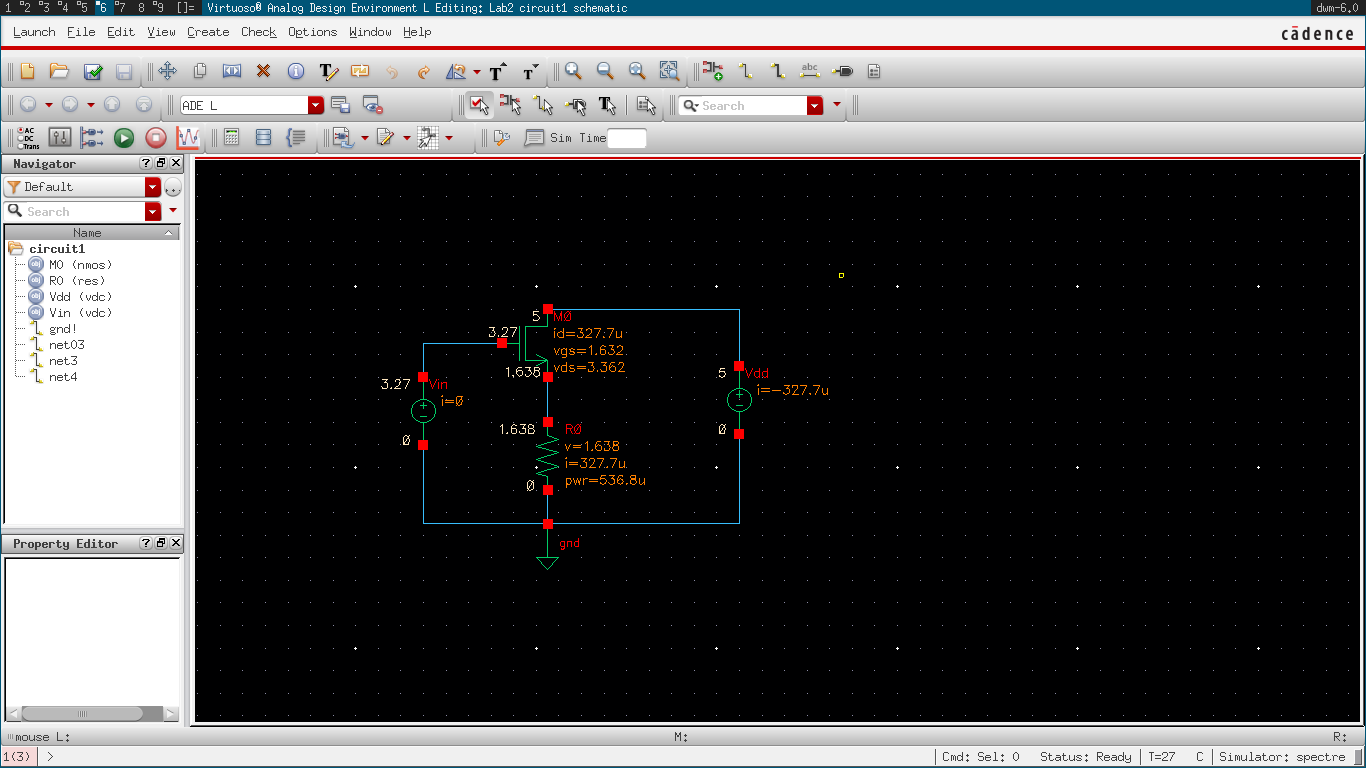
\includegraphics[scale=0.45]{../images/circuit1.PNG}
	\caption{Circuit 1}
	\label{fig:circuit1}
\end{figure}

\FloatBarrier

The circuit in figure (\ref{fig:circuit1})'s voltage transfer characteristic is acquired by sweeping $V_{in}$ from $0$\si{\volt} to $5$\si{\volt}.

\FloatBarrier

\begin{figure}[h!]
	\centering
	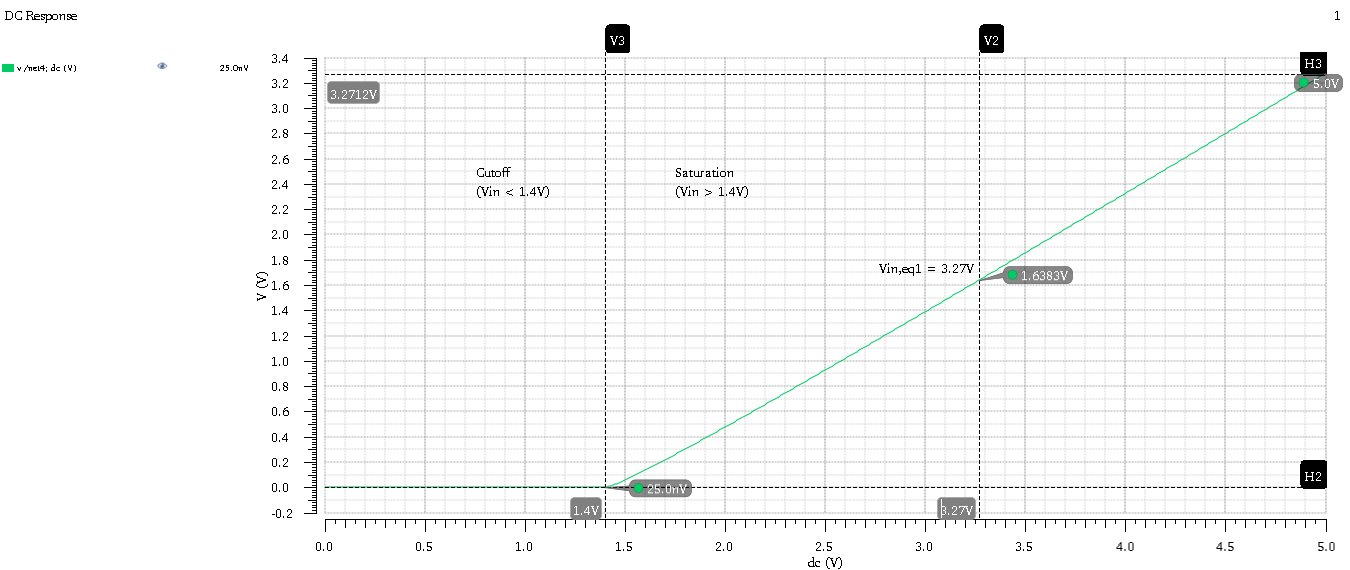
\includegraphics[scale=0.45]{../images/sim1_vtc.PNG}
	\caption{Circuit 1 Voltage Transfer Characteristic}
	\label{fig:sim1_vtc}
\end{figure}

\FloatBarrier
% Which transistor operating region corresponds to each segment of the curve?
Assume $0 < V_{in} < V_{tn}$.
% TODO Make explanation better
The transistor is in cutoff because the gate voltage is not high enough to form a channel.
For $V_{in} > V_{tn}$, the transistor turns on.
The transistor operates in saturation so long as $V_{GD} < V_{tn}$ (equivalent to $V_{DS} > V_{GS} - V_{tn}$).
Because $V_{GD} = V_{in} - 5$\si{\volt}, the transistor is in saturation so long as $V_{in} < V_{tn} + 5$\si{\volt}.
Since $V_{tn} > 0$\si{\volt} for enhancement-mode NMOSs, the transistor must be in saturation since $V_{in}$ never exceeds $5$\si{\volt}, and the transistor is not cutoff.
Here, $V_{tn} \approx 1.4$\si{\volt} since that is the dividing line between cutoff and saturation. \\

% Find V_in = V_in,eq1 that corresponds to the center of the sat region
Taking the average of the maximum and minimum values in the saturation region, $V_{in(eq1)} = 3.27$\si{\volt}.
Note that $3.27$\si{\volt} is used to compensate for the fact that $V_{out}$ at $V_{in} = 3.26$\si{\volt} is slightly below the midpoint.
% Part B: With V_in = V_in,eq1, do DC op point simulation
Figure (\ref{fig:circuit1}) shows a DC operating point simulation at this bias point.
$g_{m}$ is given by $\frac{2I_{D}'}{V_{ov}}$, where $I_{D}'$ is the saturation current not accounting for channel-length modulation and $V_{ov}$ is the overdrive voltage.
Here, the approximation $I_{D}' \approx I_{D}$ is used.

% Part C: Solve for gm and ro and compare with s.s. params in output listing
\FloatBarrier

\begin{table}[h!]
	\centering
	\caption{$g_{m}$ for the Common-Drain Amplifier}
	\label{tab:common_drain_amp_gm}
	\csvautotabular{../tables/common_drain_amp_gm.csv}
\end{table}

\FloatBarrier

$g_{ds}$ is simply the slope of the voltage transfer characteristic.
A DC operating point listing providing by Virtuoso gives the value of $g_{ds}$ for the transistor.
$r_{o}$ can then be acquired from $r_{o} = \frac{1}{g_{ds}}$.
$r_{o}$ can be calculated using $\frac{1}{\lambda I_{D}'} \approx \frac{1}{\lambda I_{D}}$.

\FloatBarrier

\begin{table}[h!]
	\centering
	\caption{$r_{o}$ for the Common-Drain Amplifier}
	\label{tab:common_drain_amp_ro}
	\csvautotabular{../tables/common_drain_amp_ro.csv}
\end{table}

\FloatBarrier
% Part D: Transient for Vin and Vout. Compare DC and AC components.

An input signal of $10$\si{\milli\volt} amplitude and $1$\si{\mega\hertz} frequency biased at $3.27$\si{\volt} is applied to the input of the common-drain amplifier.

\FloatBarrier

\begin{figure}[h!]
	\centering
	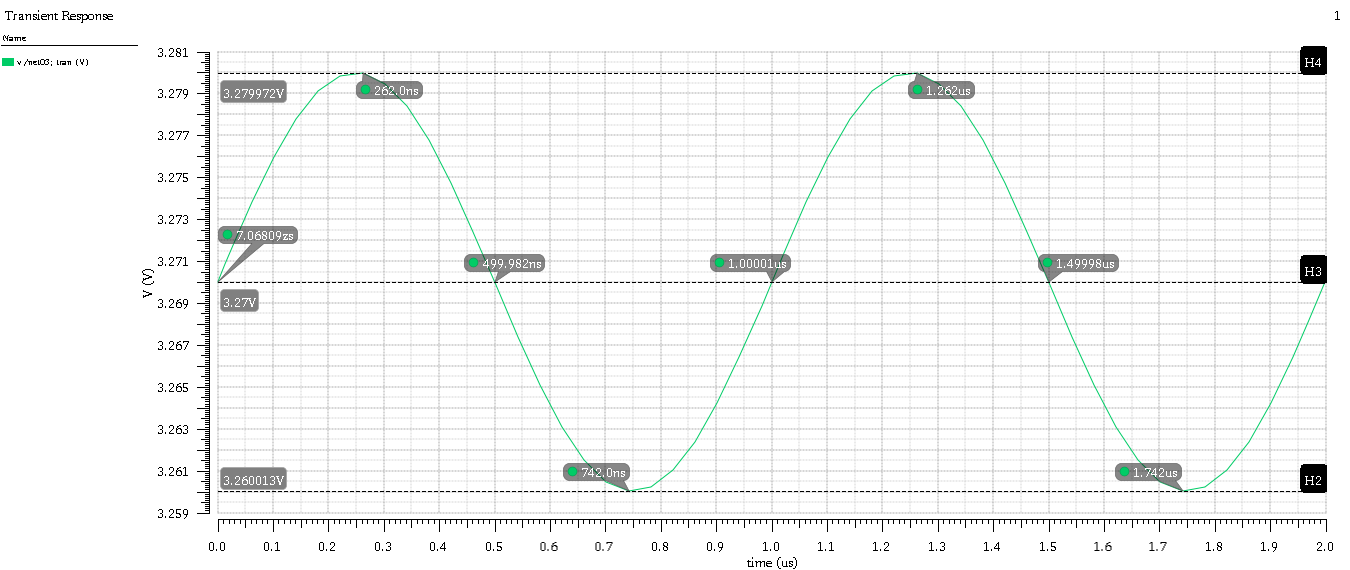
\includegraphics[scale=0.45]{../images/sim1_vin.PNG}
	\caption{$V_{in}$ for Small-Signal Analysis of Common-Drain Amplifier}
	\label{fig:sim1_vin}
\end{figure}

\FloatBarrier

A signal is then observed at the output of the amplifier.

\FloatBarrier

\begin{figure}[h!]
	\centering
	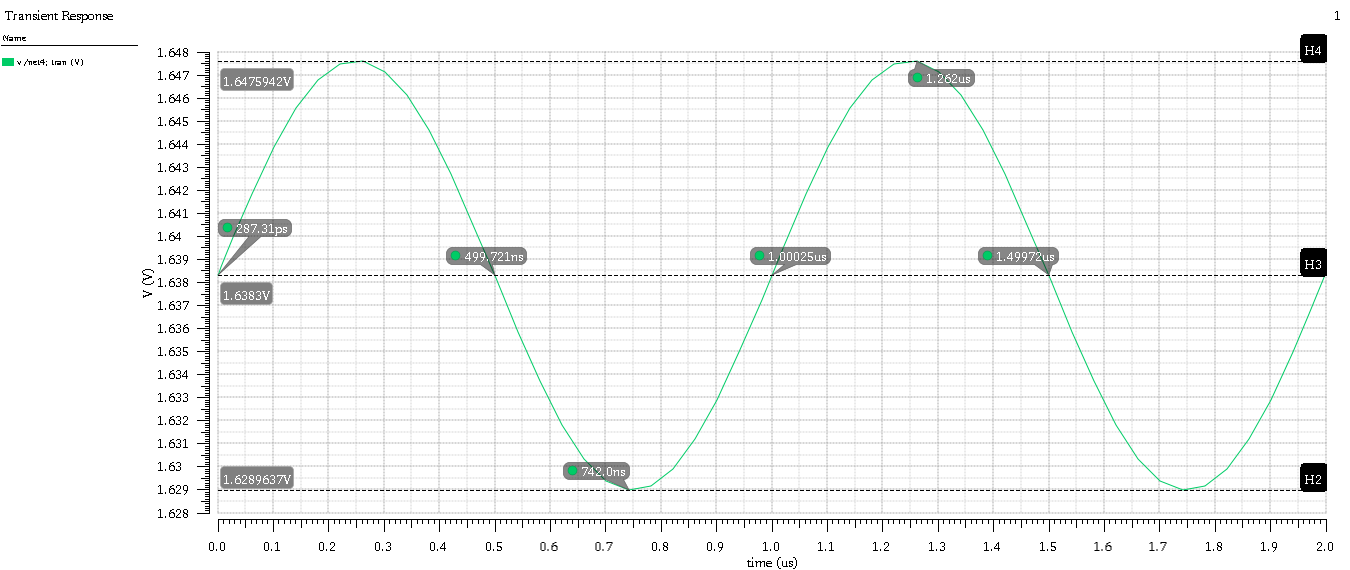
\includegraphics[scale=0.45]{../images/sim1_vout.PNG}
	\caption{$V_{out}$ for Small-Signal Analysis of Common-Drain Amplifier}
	\label{fig:sim1_vout}
\end{figure}

\FloatBarrier

The input and the output signals have the same amplitude.
This is why the common-drain amplifier is often regarded as a "voltage follower".
The bias at the output is simply the output voltage when $V_{in}$ is biased at $3.27$\si{\volt}, namely $1.64$\si{\volt}.

% Part E: Increase Vin,eq1 by 10mV. What do you observe?
$10$\si{\milli\volt} is then added to the input bias to take it from $3.27$\si{\volt} to $3.28$\si{\volt}.
Again, the output amplitude is the same as the input amplitude.
The output bias shifts up by the same amount as expected, specifically from $1.64$\si{\volt} to $1.65$\si{\volt}.
Again, this behavior is expected since the common-drain amplifier acts as a "voltage follower".
